\documentclass[10pt,french]{article}
\usepackage[utf8]{inputenc}
\usepackage[T1]{fontenc}
\usepackage[a4paper,margin=1.5cm]{geometry}
\usepackage{kpfonts}
\usepackage[dvipsnames]{xcolor}
\usepackage{mathtools,amssymb}
\usepackage[autolanguage,np]{numprint}
\usepackage{xlop}
\usepackage{cancel}
\renewcommand\CancelColor{\color{red}}
\usepackage{dsfont}
\usepackage{tkz-tab,pas-tableur}
\usepackage{babel}
\DecimalMathComma

\begin{document}
\begin{tabular}{r|p{4.5cm}}
    Rectangle & Quadrilat\`ere dont les diagonales
    sont de m\^eme longueur et
    se coupent en leur milieu.\par
    Le rectangle est un parall\'elogramme.
\end{tabular}\bigskip

\begin{tabular}{r|m{4.5cm}}
    Rectangle & Quadrilat\`ere dont les diagonales
    sont de m\^eme longueur et
    se coupent en leur milieu.\par
    Le rectangle est un parall\'elogramme.
\end{tabular}\bigskip

\begin{tabular}{r|b{4.5cm}}
    Rectangle & Quadrilat\`ere dont les diagonales
    sont de m\^eme longueur et
    se coupent en leur milieu.\par
    Le rectangle est un parall\'elogramme.
\end{tabular}\bigskip

\begin{tabular}{|m{2.5cm}|m{9cm}|m{2.5cm}|}
	\hline
		\centering 1\iere \textsc{s} & \centering  Jeudi 13 novembre \np{2014} & \centering \textbf{\'Etude de fonctions} \tabularnewline
	\hline
		\multicolumn{3}{|c|}{\textsc{Contrôle de mathématiques}} \\
	\hline
        \multicolumn{1}{|r}{\textsc{Nom}:} & \multicolumn{2}{l|}{} \\
		\multicolumn{1}{|r}{Prénom:} & \multicolumn{2}{l|}{} \\
	\hline
        \multicolumn{3}{|l|}{\bfseries Note et observations :} \\[1cm]
    \hline
\end{tabular}
\bigskip


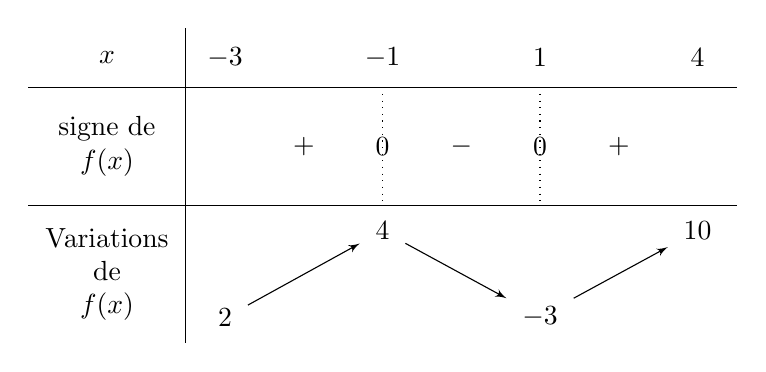
\begin{tikzpicture}
    \tkzTabInit[nocadre,espcl=2]{$x$/0.75,signe de \\ $f(x)$/1.5,Variations de \\ $f(x)$/1.75}{$-3$,$-1$,$1$,$4$}
    \tkzTabLine{,+,z,-,z,+}
    \tkzTabVar{-/$2$,+/$4$,-/$-3$,+/$10$}
\end{tikzpicture}
\bigskip

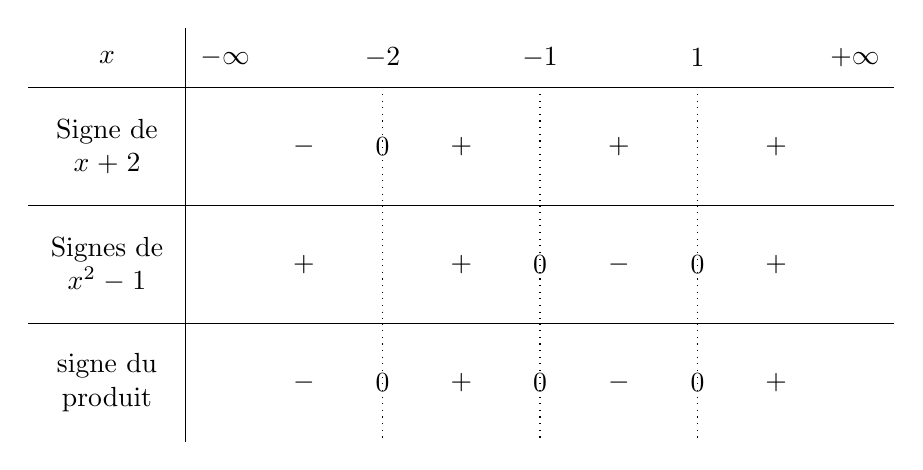
\begin{tikzpicture}
    \tkzTabInit[nocadre,espcl=2]{$x$/0.75,Signe de \\ $x+2$/1.5,Signes de \\ $x^2-1$/1.5,signe du \\ produit/1.5}{$-\infty$,$-2$,$-1$,$1$,$+\infty$}
    \tkzTabLine{,-,z,+,t,+,t,+}
    \tkzTabLine{,+,t,+,z,-,z,+}
    \tkzTabLine{,-,z,+,z,-,z,+}
\end{tikzpicture}
\bigskip

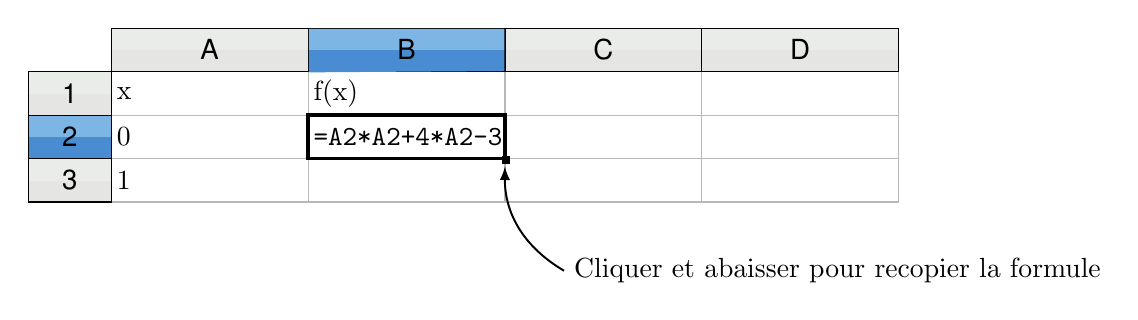
\begin{tikzpicture}
    \tabcolwidth{2.5cm}
    \tableur[3]{A-D}
    \celtxt[c]{A}{1}{x}
    \celtxt[r]{A}{2}{0}
    \celtxt[r]{A}{3}{1}
    \celtxt[c]{B}{1}{f(x)}
    \celtxt{B}{2}{=A2*A2+4*A2-3}
    \selecCell{B}{2}
    \draw[<-,>=latex,line width=0.7pt] ($(cellB-2.south east)+(0,-0.1)$) to[bend right=30] ($(cellB-2)+(2,-1.7)$)
        node[right] {Cliquer et abaisser pour recopier la formule};
\end{tikzpicture}

\end{document} 